\documentclass[../thesis.tex]{subfiles}
\begin{document}

\chapter{Theory}
\label{chp:theory}

Within this chapter the theory and procedures needed to solve a CFD case are shown. At first a broad overview is given and the generic equations are laid out. That is then followed by the explanation of the solution algorithm that is used in this work.
 
\section{Computational Fluid Dynamics}

Computational fluid dynamics or CFD in short is the computer based solving of problems regarding fluid flow, heat transfer, chemical reactions or other phenomena. The concept is used in a large variety of applications within the fields of engineering and science for at least the last 60 years \cite{versteeg2007introduction}.

Within \autoref{fig:cdf_procedure} the general procedure of solving a CFD case is shown.
\begin{figure}[htbp]
	\centering
	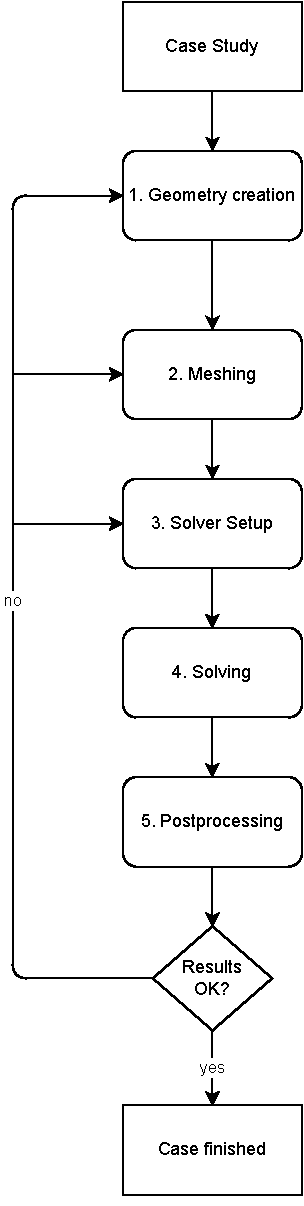
\includegraphics[scale=1.0]{CFD_general}
	\caption{CFD Case Procedure}
	\label{fig:cdf_procedure}
\end{figure}

The first step is to model the domain's geometry. In case of Ansys this step can either be done within the CFD software itself or an external CAD program. After the geometry is created or imported form an external source a mesh needs to be created. This mesh is the basis for the solver to solve the case and a vary important step. The way the mesh is set up has a significant influence on the model's results and the computational resources needed. The finer the mesh the more computational power is needed for calculating the solution. By lowering the grid's element size the resources needed or simulation time increases exponentially if everything else is kept the same.

When meshing is finished the solver has to be configured. Setting up the governing equations, simulation time and boundary conditions are steps that need to be done here for example. The hole setup is described in greater detail within \autoref{chp:model}. After the solver setup the case can be run by starting the solver. Depending on the resources needed or available this step can need some further configuration.

When the solving process has come to an end the results can be inspected. If they contain errors some of the previous done steps might need to be revisited and adapted. 

All in all solving a CFD case is an iterative process that needs to be gone through until the results look as expected and can be trusted. Further details are given in \autoref{chp:model} and \autoref{chp:limitations}.

\section{Navier-Stokes-Equations}

In this thesis the chemical reaction diffusion advection front within a radial reactor is solved using Ansys FLUENT. The basis for all this is the Lagrangian form of Newton's second law. 
\begin{equation}
	\rho \dfrac{D \textbf{u}}{D t} = - \dfrac{1}{\rho} \nabla \cdot \boldsymbol{\sigma} + \textbf{g}
\end{equation}

Within this equation $\rho$ describes the density, $\textbf{u}$ is the velocity vector, $\boldsymbol{\sigma}$ is the stress tensor and $\textbf{g}$ contains all body forces e.g. the gravity force.
With some approach to the stress vector $\boldsymbol{\sigma}$ and some coordinate transformation the Navier-Stokes-Equations in cylindrical coordinates can be derived.
The program solves the incompressible Navier-Stokes equation in cylindrical coordinates (\autoref{eqn:Navier-r} - \autoref{eqn:Navier-z}) \cite{vitturi2016navier}. The coordinates used here are the radius $r$, the height $z$ and the angle $\Theta$. $\mu$ is the viscosity and $\rho$ describes the density.

\begin{gather}
	\label{eqn:Navier-r}
	 \dfrac{\partial u_r}{\partial t} + u_r \dfrac{\partial u_r}{\partial r} + \dfrac{u_\Theta}{ r} \dfrac{\partial u_r}{\partial \Theta} - \dfrac{u_\Theta^2}{r} + u_z \dfrac{\partial u_r}{\partial z} = \\ \nonumber
	-\dfrac{1}{\rho} \dfrac{\partial p}{\partial r} + \dfrac{\mu}{\rho} \left[
		- \dfrac{u_r}{r^2} + \dfrac{1}{r} \dfrac{\partial}{\partial r} \left( r \cdot \dfrac{\partial u_r}{\partial r} \right) +
		\dfrac{1}{r^2} \dfrac{\partial^2 u_r}{\partial \Theta^2} + \dfrac{\partial^2 u_r}{\partial z^2} + \dfrac{2}{r^2} \dfrac{\partial u_\Theta}{\partial \Theta}
	\right] + g_r
\end{gather}

\begin{gather}
	\label{eqn:Navier-Theta}
	\dfrac{\partial u_\Theta}{\partial t} + u_r \dfrac{\partial u_\Theta}{\partial r} + \dfrac{u_\Theta}{ r} \dfrac{\partial u_\Theta}{\partial \Theta} - \dfrac{u_r u_\Theta}{r} + u_z \dfrac{\partial u_\Theta}{\partial z} = \\ \nonumber
	-\dfrac{1}{\rho} \dfrac{\partial p}{\partial \Theta} + \dfrac{\mu}{\rho} \left[
	- \dfrac{u_r}{r^2} + \dfrac{1}{r} \dfrac{\partial}{\partial r} \left( r \cdot \dfrac{\partial u_\Theta}{\partial r} \right) +
	\dfrac{1}{r^2} \dfrac{\partial^2 u_\Theta}{\partial \Theta^2} + \dfrac{\partial^2 u_\Theta}{\partial z^2} + \dfrac{2}{r^2} \dfrac{\partial u_r}{\partial \Theta}
	\right] + g_\Theta
\end{gather}


\begin{gather}
	\label{eqn:Navier-z}
	\dfrac{\partial u_z}{\partial t} + u_r \dfrac{\partial u_z}{\partial r} + \dfrac{u_\Theta}{ r} \dfrac{\partial u_z}{\partial \Theta} + u_z \dfrac{\partial u_z}{\partial z} = \\ \nonumber
	-\dfrac{1}{\rho} \dfrac{\partial p}{\partial z} + \dfrac{\mu}{\rho} \left[
	\dfrac{1}{r} \dfrac{\partial}{\partial r} \left( r \cdot \dfrac{\partial u_z}{\partial r} \right) +
	\dfrac{1}{r^2} \dfrac{\partial^2 u_z}{\partial \Theta^2} + \dfrac{\partial^2 u_z}{\partial z^2}
	\right] + g_z
\end{gather}

These three equations can be narrowed down for a axisymmetric case, which is used here. For this case the tangential velocity $u_\Theta = 0$. The other quantities are also not dependant of the angular position $\Theta$. Using this only two equation remain which can be written as \cite{vitturi2016navier}:

\begin{equation}
	\dfrac{\partial u_r}{\partial t} + u_r \dfrac{\partial u_r}{\partial r}+ u_z \dfrac{\partial u_r}{\partial z} = - \dfrac{1}{\rho} \dfrac{\partial p}{\partial r} +  \dfrac{\mu}{\rho} \left[ -\dfrac{u_r}{r^2} + \dfrac{1}{r} \dfrac{\partial}{\partial r} \left( r \dfrac{\partial u_r}{\partial r} \right) + \dfrac{\partial^2 u_r}{\partial z^2} \right]	+ g_r
\end{equation}

\begin{equation}
	\dfrac{\partial u_z}{\partial t} + u_r \dfrac{\partial u_z}{\partial r}+ u_z \dfrac{\partial u_z}{\partial z} = - \dfrac{1}{\rho} \dfrac{\partial p}{\partial z} + \dfrac{\mu}{\rho} \left[ \dfrac{1}{r} \dfrac{\partial}{\partial r} \left( r \dfrac{\partial u_z}{\partial r} \right) + \dfrac{\partial^2 u_z}{\partial z^2} \right]	+ g_z
\end{equation} 

In Addition to these two equations the continuity equation is given by \cite{vitturi2016navier}:

\begin{equation}
	\dfrac{1}{r} \dfrac{\partial}{\partial r}(r u_r) + \dfrac{\partial u_z}{\partial z} = 0
\end{equation}

These three equations form a system of non-linear partial differential equations. These have to be solved numerically because there is no analytical solution to this problem including given boundary conditions. The solution is generated by splitting the domain into small elements and solving the set of equations for each element to obtain a solution for the hole geometry. This method known as Finite Volume Method is described in greater detail within the following section.

\section{Finite Volume Method}

The finite Volume Method is a discretization method. It converts the set of partial differential equations into a system of linear algebraic equations \cite{darwish2021finite}. This is done in two steps. At first the partial differential equations are integrated and so transformed into balance equations \cite{darwish2021finite}. 

\subsection{Semi-Discretization}

For demonstration the conservation equation for a generic variable $ \Phi $ is given by

\begin{equation}
	\label{eqn:conserv_eq}
	\underbrace{\dfrac{\partial(\rho \Phi)}{\partial t}}_{\text{transient term}} + \underbrace{\nabla \cdot (\rho \bold{u} \Phi)}_{\text{convective term}} = \underbrace{\nabla \cdot (\Gamma_\Phi \nabla \Phi)}_{\text{diffusion term}} + \underbrace{S_\Phi}_{\text{source term}}
\end{equation}

Within this equation $ \rho $ represents the density and $ \bold{u} $ is the velocity vector. $ \nabla $ contains the spacial derivatives and $ \Gamma_\Phi $ is the diffusion coefficient of the property $ \Phi $.
For an easier explanation of the maths behind the method the steady state form of \autoref{eqn:conserv_eq} is used.

\begin{equation}
	\nabla \cdot (\rho \bold{u} \Phi) = \nabla \cdot (\Gamma_\Phi \nabla \Phi) + S_\Phi
\end{equation}

As already stated this equation is integrated over the control volume shown in \autoref{fig:FVM_CV} witch leads to \autoref{eqn:FVM_volint}.

\begin{equation}
	\label{eqn:FVM_volint}
	\int_{V_C} \nabla \cdot (\rho \bold{u} \Phi) dV = \int_{V_C} \nabla \cdot (\Gamma_\Phi \nabla \Phi) dV + \int_{V_C} S_\Phi dV
\end{equation}

The volume integrals, within the convective and diffusive term, can be replaced by surface integrals using the divergence theorem. That leads to the semi-discretized \autoref{eqn:FVM_Aint}.

\begin{equation}
	\label{eqn:FVM_Aint}
	\oint_{\partial V_C} (\rho \bold{u} \Phi) d\bold{S} = \oint_{\partial V_C} (\Gamma_\Phi \nabla \Phi) d\bold{S} + \int_{V_C} S_\Phi dV
\end{equation}

The variable $ \bold{S}$ is the surface vector, the operator ($\cdot$) is the dot product and $ \oint_{\partial V_C}$ is the surface integral operator.

\subsection{Surface Integration}

As seen in \autoref{eqn:FVM_Aint} surface integrals are needed to calculate the value of the property $\Phi$ for the control volume. Theses surface integrals can be split into a summation over each cell surface. This step can be done for the convective term shown in \autoref{eqn:conv_sint} as well as for the diffusion term shown in \autoref{eqn:diffu_sint}.

\begin{equation}
	\label{eqn:conv_sint}
	\oint_{\partial V_C} (\rho \bold{u} \Phi) d\bold{S} = \sum_{f_i}^{n_{\text{faces}}}\left( \int_{f} (\rho \bold{u} \Phi) d\bold{S} \right)
\end{equation}

\begin{equation}
	\label{eqn:diffu_sint}
	\oint_{\partial V_C} (\Gamma_\Phi \nabla \Phi) d\bold{S} =  \sum_{f_i}^{n_{\text{faces}}}\left( \int_{f} (\Gamma_\Phi \nabla \Phi) \right)
\end{equation} 

\begin{figure}[htbp]
	\centering
	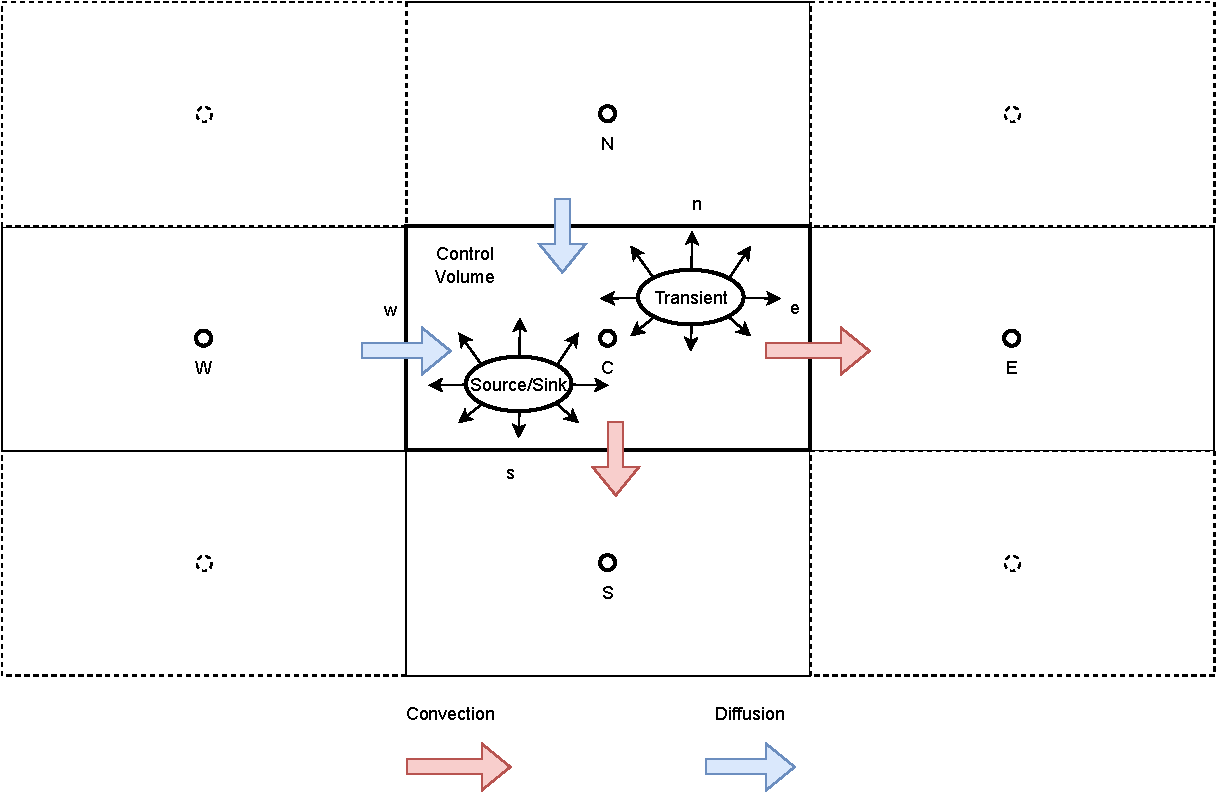
\includegraphics[scale=0.70]{Control_Volumen}
	\caption{Control Volume example}
	\label{fig:FVM_CV}
\end{figure}

From this point on it can be seen that the values of $\Phi$ at each cells surface are needed. The solution algorithm used calculates and stores the results only at the cells centre. To obtain values at the cell's surfaces the neighbouring cell's values are used as well. The method used here is called Quadratic upwind differencing scheme (QUICK) and is explained in greater detail within the following section.

\subsection{Quadratic upwind differencing scheme}
\label{sec:QUICK}

As shown in \autoref{fig:FVM_CV} each cell in a 2D case has 4 neighbouring cells that are labelled N for north, S for south, E for east and W for West. The QUICK method uses the 2 neighbouring cells upward the flow direction. A schematic is shown in \autoref{fig:QUICK}. The cell westward to the W cell is called WW and using the same naming scheme the cell eastward to E is named EE.

\begin{figure}[htbp]
	\centering
	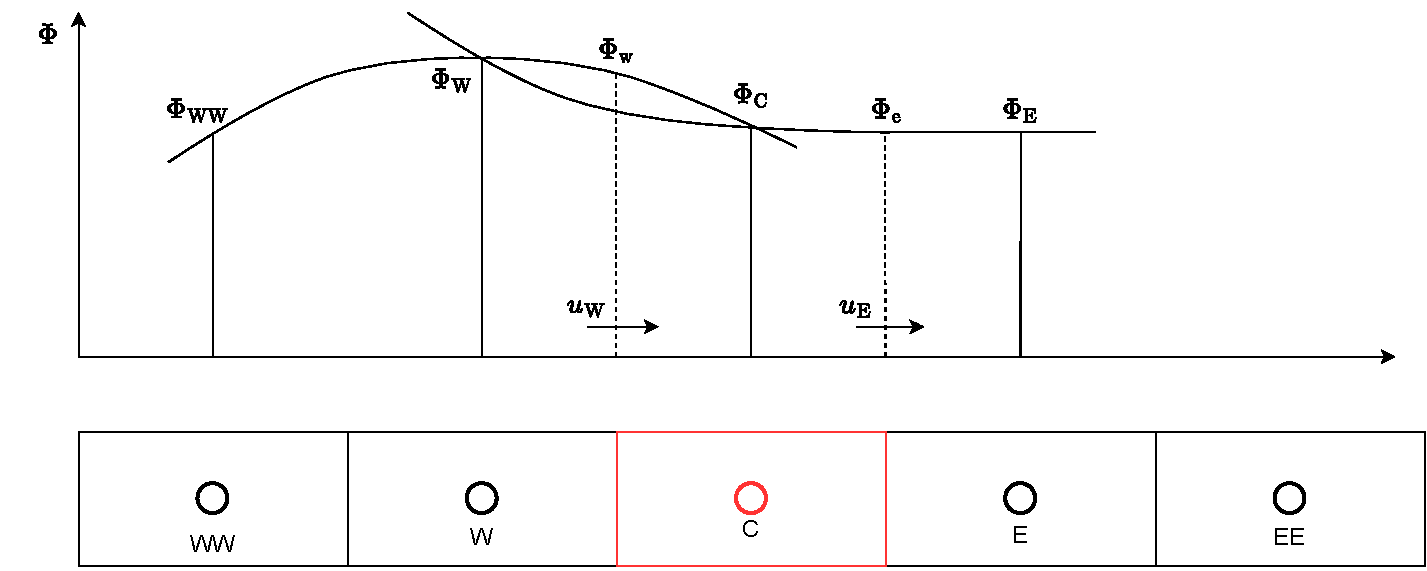
\includegraphics[scale=0.6]{QUICK}
	\caption{QUICK method cell scheme}
	\label{fig:QUICK}
\end{figure}

With a flow from west to east through the Cell with it's centre C the cells surface values $\Phi_w$ for the west facing surface and $\Phi_e$ for the east facing surface are calculated as follows \cite{versteeg2007introduction}:

\begin{equation}
	\Phi_w = \dfrac{6}{8} \Phi_W + \dfrac{3}{8} \Phi_P - \dfrac{1}{8} \Phi_{WW}
\end{equation}
\begin{equation}
	\Phi_e = \dfrac{6}{8} \Phi_P + \dfrac{3}{8} \Phi_E - \dfrac{1}{8} \Phi_{W}
\end{equation}

If the flow is reverse in direction the method stays the same but the cells the values are used from do change.

\begin{equation}
	\Phi_w = \dfrac{6}{8} \Phi_P + \dfrac{3}{8} \Phi_W - \dfrac{1}{8} \Phi_{E}
\end{equation}
\begin{equation}
	\Phi_e = \dfrac{6}{8} \Phi_E + \dfrac{3}{8} \Phi_P - \dfrac{1}{8} \Phi_{EE}
\end{equation}

\section{Solution Method}
\label{sec:sol_method}

The solution method used in this case is called PISO algorithm which stands for Pressure Implicit with Splitting Operation algorithm. A general overview of the method's procedure can bes seen in \autoref{fig:PISO}.

\begin{figure}[htbp]
	\centering
	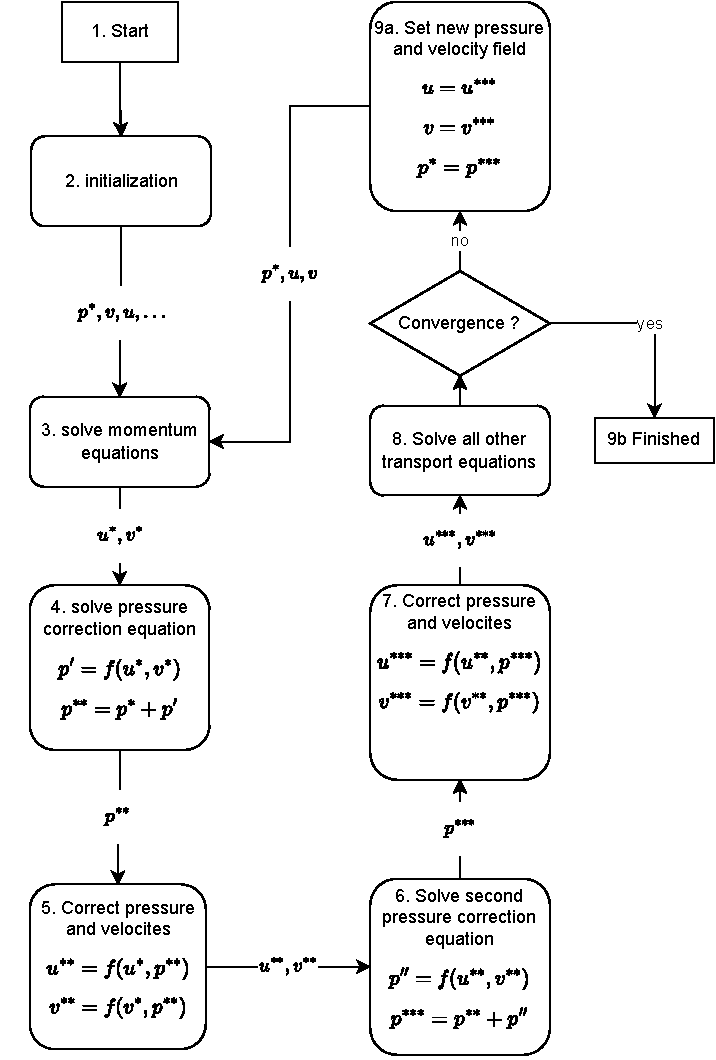
\includegraphics[scale=1.0]{PISO}
	\caption{PISO algorithm}
	\label{fig:PISO}
\end{figure}

At first all fields have to be initialized with some values by the user. With this initial values the method starts it's calculation. The first step within the calculation is to get the results of the momentum equations for each cell within the mesh. The results gained are, a 2D case given, the velocity fields $v^*$ and $u^*$. After this step is finished the gained velocity fields are used to calculate the pressure correction $p'$. This is done by setting the pressure offset to a value that satisfies the continuity equation for the cell. With this offset $p'$ a new pressure field $p^{**}$ can be calculated that is then used to correct the velocity fields $u^*$ and $v^*$. This correction is done in a way similar to the already described method in \autoref{sec:QUICK} using the values of the neighbouring cells. After the new velocity fields $u^{**}$ and $v^{**}$ have been gained the PISO algorithm performs a second pressure correction. This yields the pressure field $p^{***}$. Now a second velocity field correction takes place in the same manner as the first one. After that is done all other transport equations are solved using the latest fields for the velocities $u^{***}$, $v^{***}$ and the pressure $p^{***}$. Finally a convergence check is performed and if success full the algorithm stops. The convergence is a criterium that does a comparison of the fields that are given as input and the ones yielded as output. If the difference is bellow a certain threshold the solution has converged. The threshold as to be given by the user for each variable of interest or the default ones are used. If the resulting fields have not converged the latest output is used as new input and the solving and corrections steps take place again. This iterative approach is done as long as the convergence criterium is not fulfilled or the maximum amount of iterations is reached.


\section{Fluid Phenomena}

Within a developing reaction-diffusion-advection front some specific phenomena take place. The main ones are looked at in this section.

\subsection{Taylor-Dispersion}

The first phenomenon taking place within a reaction-diffusion-advection front is called Taylor-Dispersion. This was first discovered by G.I. Taylor\cite{aris1956dispersion} in 1956. The discovered phenomenon describes the spreading of the front over time as it can be seen within \autoref{fig:taylor-disp} \cite{levenspiel1998chemical}. 

\begin{figure}[htbp]
	\centering
	\includegraphics[scale=0.8]{taylor-dispersion}
	\caption{Taylor dispersion}
	\label{fig:taylor-disp}
\end{figure}

As shown the front's concentration distribution changes along the flow direction $x$ within time $t$. The peak lowers and the distribution widens as time passes. How quickly this effect takes place and which parameters have a significant influence is discussed within \autoref{chp:}. Within this work the front's width as well as the height averaged concentration distribution are the results looked at when checking this phenomenon.

\end{document}